
\label{sec:app}
%\subsection{Overview}
Figure~\ref{fig:app} shows the overview of our approach.
For each HTML element rendered on the webpage, we calculate the performance cost on it including the wall-clock real-time cost and relative cost towards the database size. This performance information will be displayed on the webpage after it's loaded inside the Browser. And then, for each HTML element, we provide the possible design opportunities. Once developers choose one design opportunity for certain HTML element, the source code will be edited to satisfy the developers' requirement.
\begin{figure}[H]
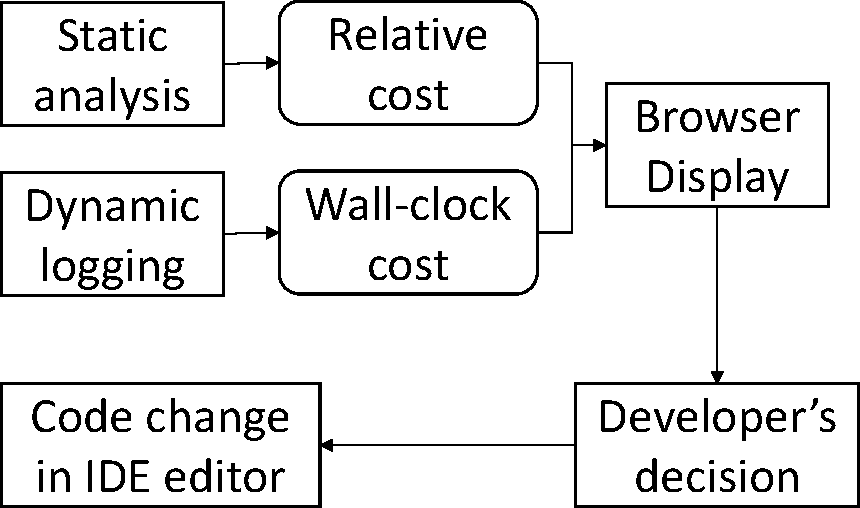
\includegraphics[width=\columnwidth]{figs/p2-crop.pdf}
\caption{Overview of Approach}
\label{fig:app}
\end{figure}
\subsection{Performance Cost Estimation}
We estimates the performance cost for each HTML tag that will be rendered on the page through dynamic run-time logging and static analysis, which is a new granularity for performance estimation. Also our approach includes the wall-clock performance cost and relative performance cost towards the database size. As a result, this approach also works when there is not a representative workload for us to gain enough performance cost information. 
 
\subsection{Interactive Design Interface}
We propose a brand new interface for web application design. We firstly render the performance cost information estimated from last step on the web page for each HTML tag. And for those HTML tags that take large performance cost, we identify the possible alternative design choices from these options: (1) pagination, (2) approximation, (3) asynchronous loading, and (4) removing. Developers are allowed to choose their desired design choice. After developers' selection, source code will be automatically revised so that the application can achieve their wanted behavior. The performance cost of updated application will re-estimated and displayed on the web page in order that the performance improvement can be observed. 



